\documentclass[border=3.5pt]{standalone} %,outext=.png ,convert={density=300,size=1080x1090}
\usepackage{tikz}
%\usepackage{tikz-graph}
%\usetikzlibrary{arrows.meta}
\usepackage{filecontents}
\usepackage{tikz, xcolor}
\usetikzlibrary{shapes,arrows,arrows.meta}
\usetikzlibrary{er,positioning}
\usetikzlibrary{calc}
\usetikzlibrary{decorations.pathreplacing,decorations.markings}
\usepackage{times}

\newcommand{\midarrow}{\tikz \draw[-triangle 90] (0,0) -- +(.1,0);}

% set up externalization
%\usetikzlibrary{external}
%\tikzset{external/system call={latex \tikzexternalcheckshellescape -halt-on-error
%-interaction=batchmode -jobname "\image" "\texsource";
%dvips -o "\image".ps "\image".dvi;
%ps2eps "\image.ps"}}
%\tikzexternalize

\tikzset{%
%  multi attribute/.style={attribute,double distance=1.5pt},
%  derived attribute/.style={attribute ,dashed},
%  total/.style={double distance=1.5pt},
%  every entity/.style={draw=orange, fill=orange!20},
%  every attribute/.style={draw=MediumPurple1, fill=MediumPurple1!20},
%  every relationship/.style={draw=Chartreuse2, fill=Chartreuse2!20},
  %every node/.style={inner sep=0,outer sep=0},
     % style to apply some styles to each segment of a path
  on each segment/.style={
    decorate,
    decoration={
      show path construction,
      moveto code={},
      lineto code={
        \path [#1]
        (\tikzinputsegmentfirst) -- (\tikzinputsegmentlast);
      },
      curveto code={
        \path [#1] (\tikzinputsegmentfirst)
        .. controls
        (\tikzinputsegmentsupporta) and (\tikzinputsegmentsupportb)
        ..
        (\tikzinputsegmentlast);
      },
      closepath code={
        \path [#1]
        (\tikzinputsegmentfirst) -- (\tikzinputsegmentlast);
      },
    },
  },
  % style to add an arrow in the middle of a path
  mid arrow/.style={postaction={decorate,decoration={
        markings,
        mark=at position .5 with {\arrowreversed[#1]{stealth'}}
      }}},
  loop/.style={ % requires library shapes.misc
        draw,
        chamfered rectangle,
        chamfered rectangle xsep=2cm
    },
}

\tikzstyle{process} = [loop, draw, text width=4cm,
                        text centered, node distance=0.625cm,
                        inner sep=0pt, minimum height=1cm,minimum width=4cm]
\tikzstyle{data} = [rectangle, draw, text width=3cm,
                     text centered, rounded corners,
                      minimum height=1cm,minimum width=3.cm,node distance=0.625cm,]
\tikzstyle{line} = [draw, -latex']
\tikzstyle{parameters} = [draw, rectangle, node distance=0.625cm, minimum height=1cm,minimum width=2cm]
\tikzstyle{blank} = [node distance=0.625cm]

\begin{document}

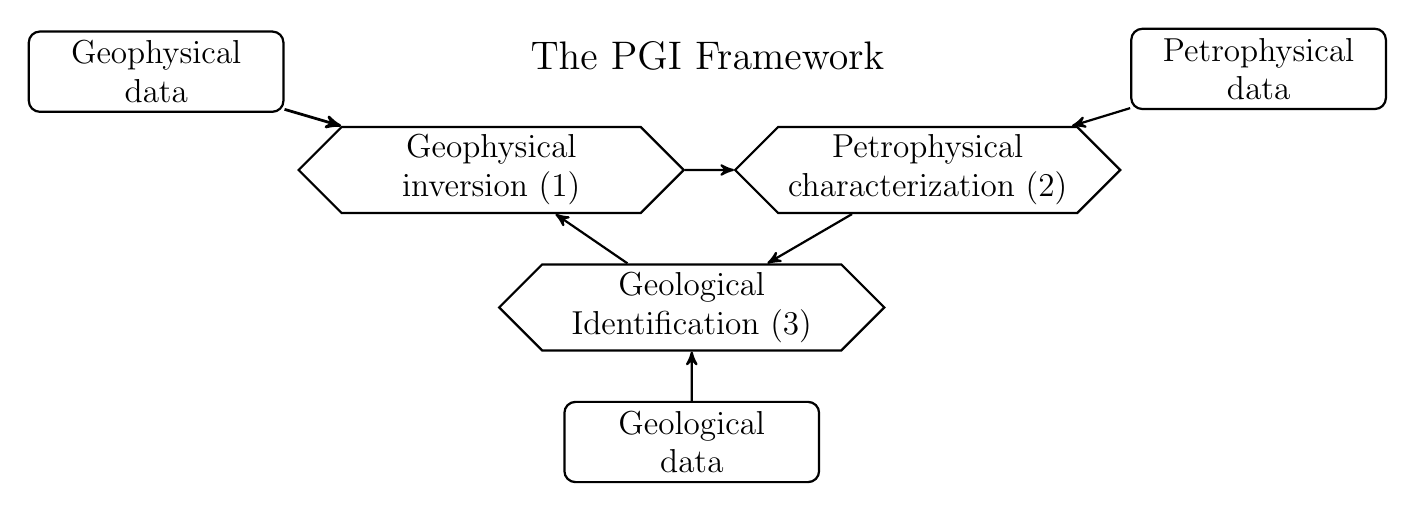
\begin{tikzpicture}[shorten >=0pt,auto,node distance=0.5cm,font=\large,
                thick,main node/.style={circle,draw}] %[node distance = 10cm, auto,->,>=stealth',]font=\Large\bfseries
    % Place nodes
    \node [process, align=center] (Inversion) {\large Geophysical\\inversion (1)};
    \node [data,above left= of Inversion,  align=center] (GeoPhyData) {\large Geophysical\\data};
    %\node [parameters, right = of Inversion,  align=center,] (M) {\large Geophysical\\\large model $\mathbf{m}$};
    \node [process,right = of Inversion,  align=center] (ExpMap) {\large Petrophysical\\characterization (2)};
    \node [data, above right= of ExpMap,  align=center, text width=3cm] [xshift=-0.15em, yshift=0.1em] (PetroData) {\large Petrophysical \\\large data};
    %\node [parameters, below =  of ExpMap, align=center,] (PetroDis) {\large Petrophysical\\\large distribution $\mathcal{M}$};
    \node [process, below left =of ExpMap, align=center] (Classification) [xshift=5.15em, yshift=-2.1em] {\large Geological\\Identification (3)};
    %\node [parameters, below = of Inversion,  align=center] (Mref) {\large $\mathbf{m}_{ref}, W_s$};
    \node [data, below = of Classification, align=center, text width=3cm] (Geodata) {\large Geological\\\large data};
    %\node [process, left = of Inversion, align=center] (StoppingCriteria) {\large Stopping\\\large criteria};
    %\node [data, left= of GeoPhyData, above= of StoppingCriteria,  align=center] (Initialization) [xshift=0em, yshift=0.6em] {\large Initialization\\$\mathbf{m}_0$, $\Theta_0$,$\mathbf{z}_0$};
    %\node [data, below left= of Mref, align=center] (Output) [xshift=0em, yshift=-0.3em] {\large Final \large output\\$\mathbf{m}$, $\Theta$,$\mathbf{z}$};
    %\node[main node] (2) [below left of=1] {2};
    %\node[main node] (3) [below right of=1] {3};

    % invisible node
    %\node[inner sep=0,minimum size=0,below left of=StoppingCriteria] (k) {};

    \path [->,>=stealth',line width =1pt] (GeoPhyData) edge node [xshift=0em, yshift=-.4em] {} (Inversion);
    \path [->,>=stealth',] (Inversion) edge node [xshift=-.7em, yshift=0.55em] {} (ExpMap);
    %\path [->,>=stealth',] (M) edge node [xshift=0.5em, yshift=0.55em] {Input} (ExpMap);
    \path [->,>=stealth',] (PetroData) edge node [xshift=0em, yshift=-.2em] {} (ExpMap);
    \path [->,>=stealth',] (ExpMap)  edge node {} (Classification);
    %\path [->,>=stealth',] (PetroDis) edge node [xshift=-0.35em, yshift=-.3em] {Rules} (Classification);
    \path [->,>=stealth',] (Classification) edge node [xshift=.2em, yshift=0em] {} (Inversion);
    %\path [->,>=stealth',] (Mref) edge node {Prior} (Inversion);
    %\path [->,>=stealth',] (M) edge node {Input} (Classification);
    \path [->,>=stealth',] (Geodata) edge node [xshift=.2em, yshift=0.2em] {} (Classification);
    %\path [->,>=stealth',] (Initialization) edge node [xshift=.0em, yshift=-0.5em] {Check} (StoppingCriteria);
    %\path [->,>=stealth',] (StoppingCriteria) edge node {No} (Inversion);
    %\path [->,>=stealth',to path={|- (\tikztotarget) \tikztonodes}] (StoppingCriteria.west) edge node [xshift=1em, yshift=7.5em] {Yes} (Output.west);
    %\path [->,>=stealth', to path={-| (\tikztotarget) \tikztonodes}] (Mref) edge node [xshift=2em, yshift=-1em] {Check} (StoppingCriteria);

    %\draw[black,thick,dotted,,postaction={on each segment={mid arrow={black,scale=2}}}] ($(Inversion.north west)+(-0.3,.5)$) rectangle ($(Classification.south est)+(3.,-.8)$);
    \node [blank,font =\Large, align=center, yshift=-1em] (Process) at (current bounding box.north) {The PGI Framework};

    %\draw[red,thick,dashed]($(Classification.north west)+(-0.3,.5)$) rectangle ($(Geodata.south est)+(.825,-.8)$);

    %\node[diamond,draw,black, below = of Mref,minimum width=1mm,minimum %height=1mm,](d){};%
    %\node[anchor=west,%right= of d](dt){Process};%
%
%    %\node[rectangle,draw,black rounded corners, right = of dt,minimum %width=1mm,minimum height=1mm,](r){};%
    %\node[anchor=west,right= of r](rt){D%ata};%
%
%    %\node[circle,draw,black right = of rt ,minimum width=1mm,minimum %height=1mm](c){};%
    %\node[anchor=west,right= of c](ct){Parameters};%
%
    %\node[draw,fit=(ct)(c)(dt)(d)(rt)(r)] {};

    %\path[draw=blue,dotted,thick,line width = 1pt,postaction={on each segment={mid arrow={red,scale=2}}}] ($(Inversion.north west)+(-1,1)$) -- ($(ExpMap.north east)+(1,1)$) -- ($(PetroDis.south east)+(1,-1)$) -- ($(Mref.south west)+(-1,-1)$) -- ($(Inversion.north west)+(-1,1)$);

    %\begin{scope}[very thick, every node/.style={sloped,allow upside down}]
  %\draw (-4,0)-- node {\midarrow} (4,0);
  %\draw (4,0)-- node {\midarrow} (4,2);
  %\draw (4,2)-- node {\midarrow} (-4,2);
  %\draw (-4,2)-- node {\midarrow} (-4,0);
    %\end{scope}
\end{tikzpicture}

\end{document}
